\documentclass{beamer}
% Prévoir à peu près un transparent par minute d'exposé.
% Deux ou trois sections semble être une bonne chose.
\mode<presentation>
{
	\usetheme{Warsaw}
	\setbeamercovered{highly dynamic}
	\setbeamercovered{invisible}
}

\usepackage[english]{babel}
\usepackage[utf8]{inputenc}
%\usepackage{hyperref}

\setbeamersize{text margin left=20pt}
\setbeamersize{text margin right=20pt}

\defbeamertemplate*{footline}{infolines theme}
{
	\leavevmode%
	\hbox{%
		\begin{beamercolorbox}[wd=.33\paperwidth,ht=2.25ex,dp=1ex,center]{author in head/foot}%
			\usebeamerfont{author in head/foot}G. Lesauvage
		\end{beamercolorbox}%
		\begin{beamercolorbox}[wd=.33\paperwidth,ht=2.25ex,dp=1ex,center]{title in head/foot}%
			\usebeamerfont{title in head/foot}\insertshorttitle
		\end{beamercolorbox}%
		\begin{beamercolorbox}[wd=.33\paperwidth,ht=2.25ex,dp=1ex,right]{date in head/foot}%
			\usebeamerfont{date in head/foot}3 mars 2011\hspace*{2em}
			\insertframenumber{}/\inserttotalframenumber\hspace*{2ex}
		\end{beamercolorbox}
	}%
	\vskip0pt%
}

\date{\tiny 2-4 mars 2011}
\title[ROADEF 2011]
{
	$D^2CTS$ : un simulateur de terminal à conteneurs
}

\author
{
	S. Balev, F. Guinand et G. Lesauvage
}

\institute[LITIS]
{
	
 \begin{columns}
 		\begin{column}[l]{6cm}
 			\begin{center}
 			
\includegraphics[height=.1\textheight]{fig/logouniversiteduhavre.png} \\
 			\tiny\textit{Unit\'{e} de Formation et de Recherche des Sciences et Techniques}
 			\end{center}
 		\end{column}
 		\begin{column}[r]{6cm}
 			\begin{center}
 			
\includegraphics[height=.135\textheight]{fig/logolitis.png} \\
 			\tiny\textit{Laboratoire d'Informatique et du Traitement de l'Information et des Syst\`{e}mes}
 			\end{center}
 		\end{column}
 \end{columns}

 	
}

\normalsize

  \AtBeginSection[Plan]
  {
  \begin{frame}<beamer>
  \frametitle{Plan}
  \tableofcontents[currentsection]
  \end{frame}
  }
\setbeamertemplate{blocks}[rounded][shadow=true]
\subject{ROADEF 2011 Saint Etienne}
\begin{document}

\begin{frame}
\titlepage
\end{frame}

\begin{frame}
\frametitle{Plan}
\tableofcontents
\end{frame}

\section{Présentation et objectifs}
\begin{frame}{Le projet CALAS}
\begin{columns}
    \begin{column}[l]{5.5cm}	
	\begin{itemize}
		\item Système de mesure laser

		\item Entreprises : 
			\begin{itemize}
			 \item LDTT
	 		 \item EADS/Astrium
			\end{itemize}

		\item Laboratoires : 
			\begin{itemize}
			    \item LMAH
			    \item LITIS
			\end{itemize}
	\end{itemize}
    \end{column}
    \begin{column}[r]{4.5cm}
		\begin{flushright}
		  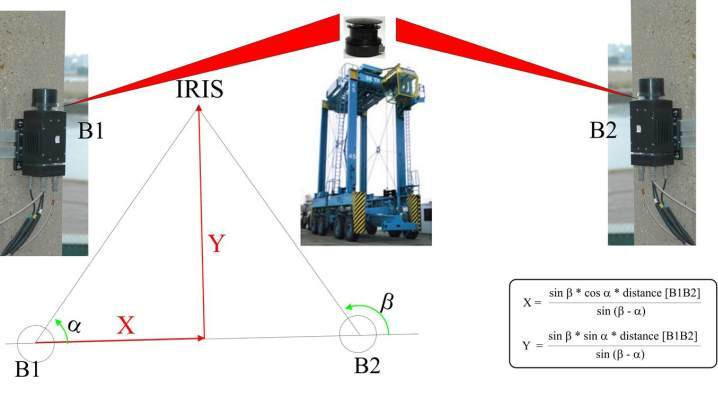
\includegraphics[height=.30\textheight]{fig/angles.jpg}
		\end{flushright}
    \end{column}
 \end{columns}	
  \pause
  \begin{block}{Objectifs du projet CALAS : }
		\begin{minipage}[]{\columnwidth}
			Connaître l'état du terminal en temps réel, c'est-à-dire à la fois la position des conteneurs et celle des engins de manutention.
		\end{minipage}
	\end{block}
	

\end{frame}

\begin{frame}{$D^2CTS$}

  Dynamic and Distributed Container Terminal Simulator : simulateur dynamique et distribué de terminal à conteneurs
  \begin{block}{Objectif : }
   	\begin{minipage}[]{\columnwidth}
		Simuler un terminal à conteneurs à la fois dans sa structure et dans sa dynamique
	\end{minipage}
  \end{block}
  \begin{block}{But final : }
   	\begin{minipage}[]{\columnwidth}
		Mettre à l'épreuve différents algorithmes d'optimisation du terminal dans des conditions réalistes
	\end{minipage}
  \end{block}
\end{frame}

\section{Modélisation}
  \subsection{Structure}
 \begin{frame}{Exemple de terminal : le Terminal de Normandie (PAH)}
   \begin{center}
	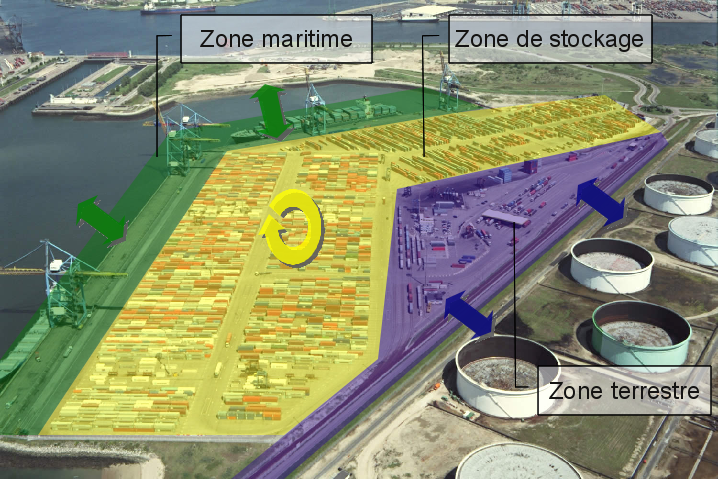
\includegraphics[height=.60\textheight]{fig/3zonesDuTN.png}
  \end{center}   
 \end{frame}


  \begin{frame}{Graphe routier}
\begin{columns}
    \begin{column}[l]{4.0cm}	
	\begin{itemize}
	  \item Carefours
	  \item Routes
	  \item Points de route
	  \item Travées
	  \item Points de travées
	\end{itemize}
    \end{column}
    \begin{column}[r]{6.5cm}
	\begin{flushright}
	  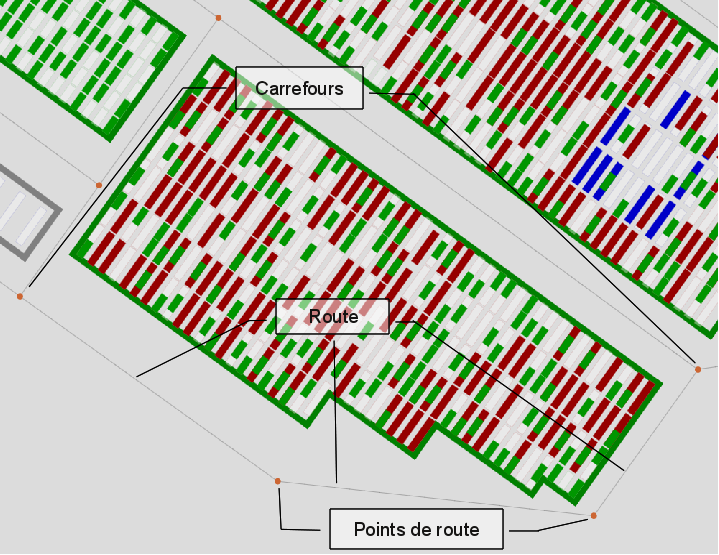
\includegraphics[height=.55\textheight]{fig/FigPointsDeRoute.png}
	\end{flushright}
    \end{column}
 \end{columns}	
    
 \end{frame}

\subsection{Système de localisation laser}
\begin{frame}{Système de localisation laser}
  \begin{columns}
    \begin{column}[l]{4.0cm}	
	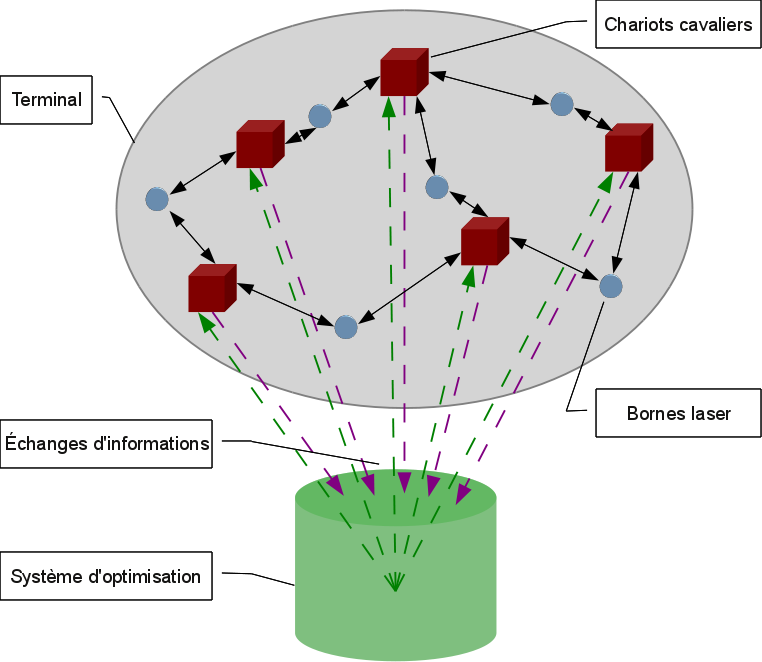
\includegraphics[height=.50\textheight]{fig/communications.png}
	\begin{center}
	   \tiny \textit{Communications entre les chariots cavaliers et le système d'optimisation}
	  \end{center}
    \end{column}
    \begin{column}[r]{6.5cm}
	\begin{flushright}
	  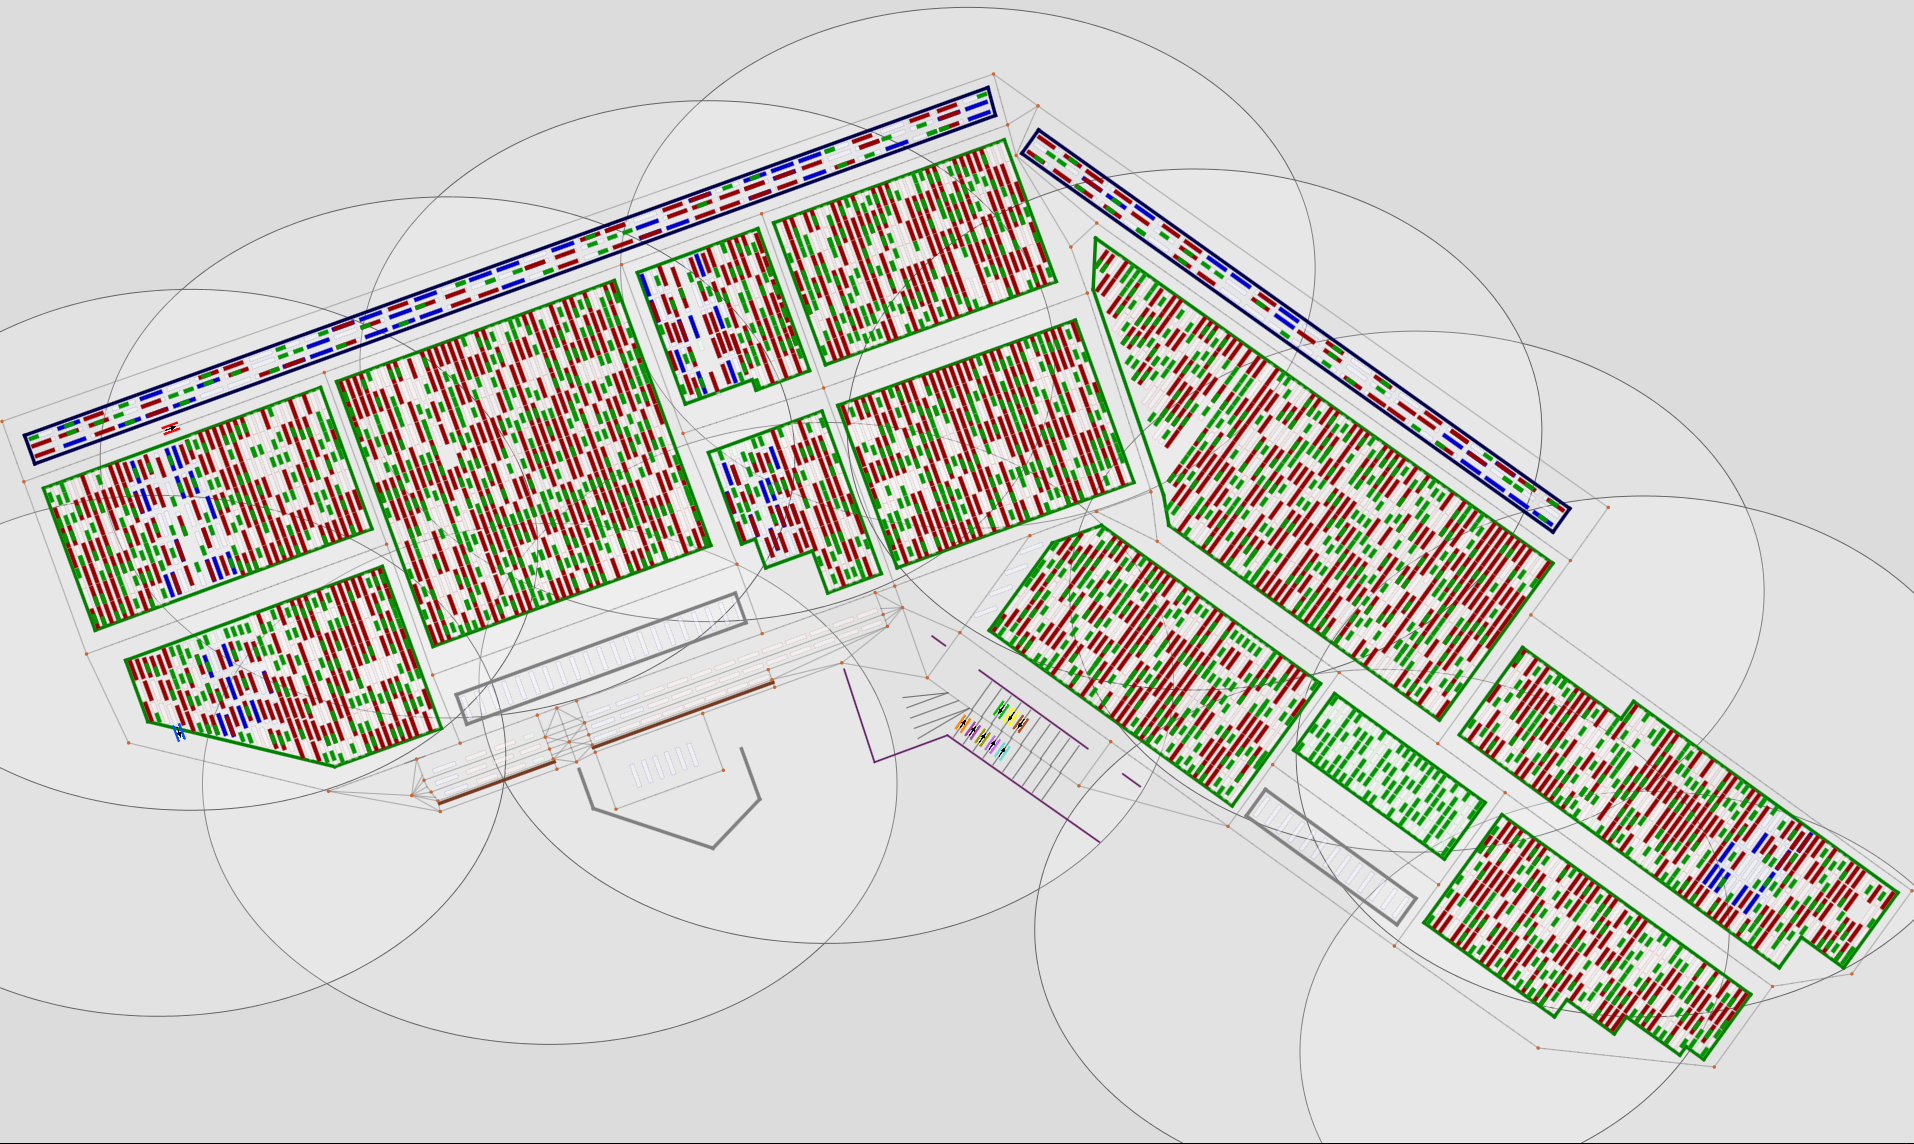
\includegraphics[height=.50\textheight]{fig/captureBornesLaser.png}
	  \begin{center}
	   \tiny \textit{ Modélisation du système de localisation laser sur le Terminal de Normandie (PAH)}
	  \end{center}
	\end{flushright}
    \end{column}
 \end{columns}	
\end{frame}

 \subsection{Mobilité}
  \begin{frame}{Mobilité}
  
  \begin{center}
  La mobilité dans le simulateur ne concerne que les chariots cavaliers pour le moment
\vspace{0.8cm}

\begin{columns}
    \begin{column}[l]{3.0cm}	
      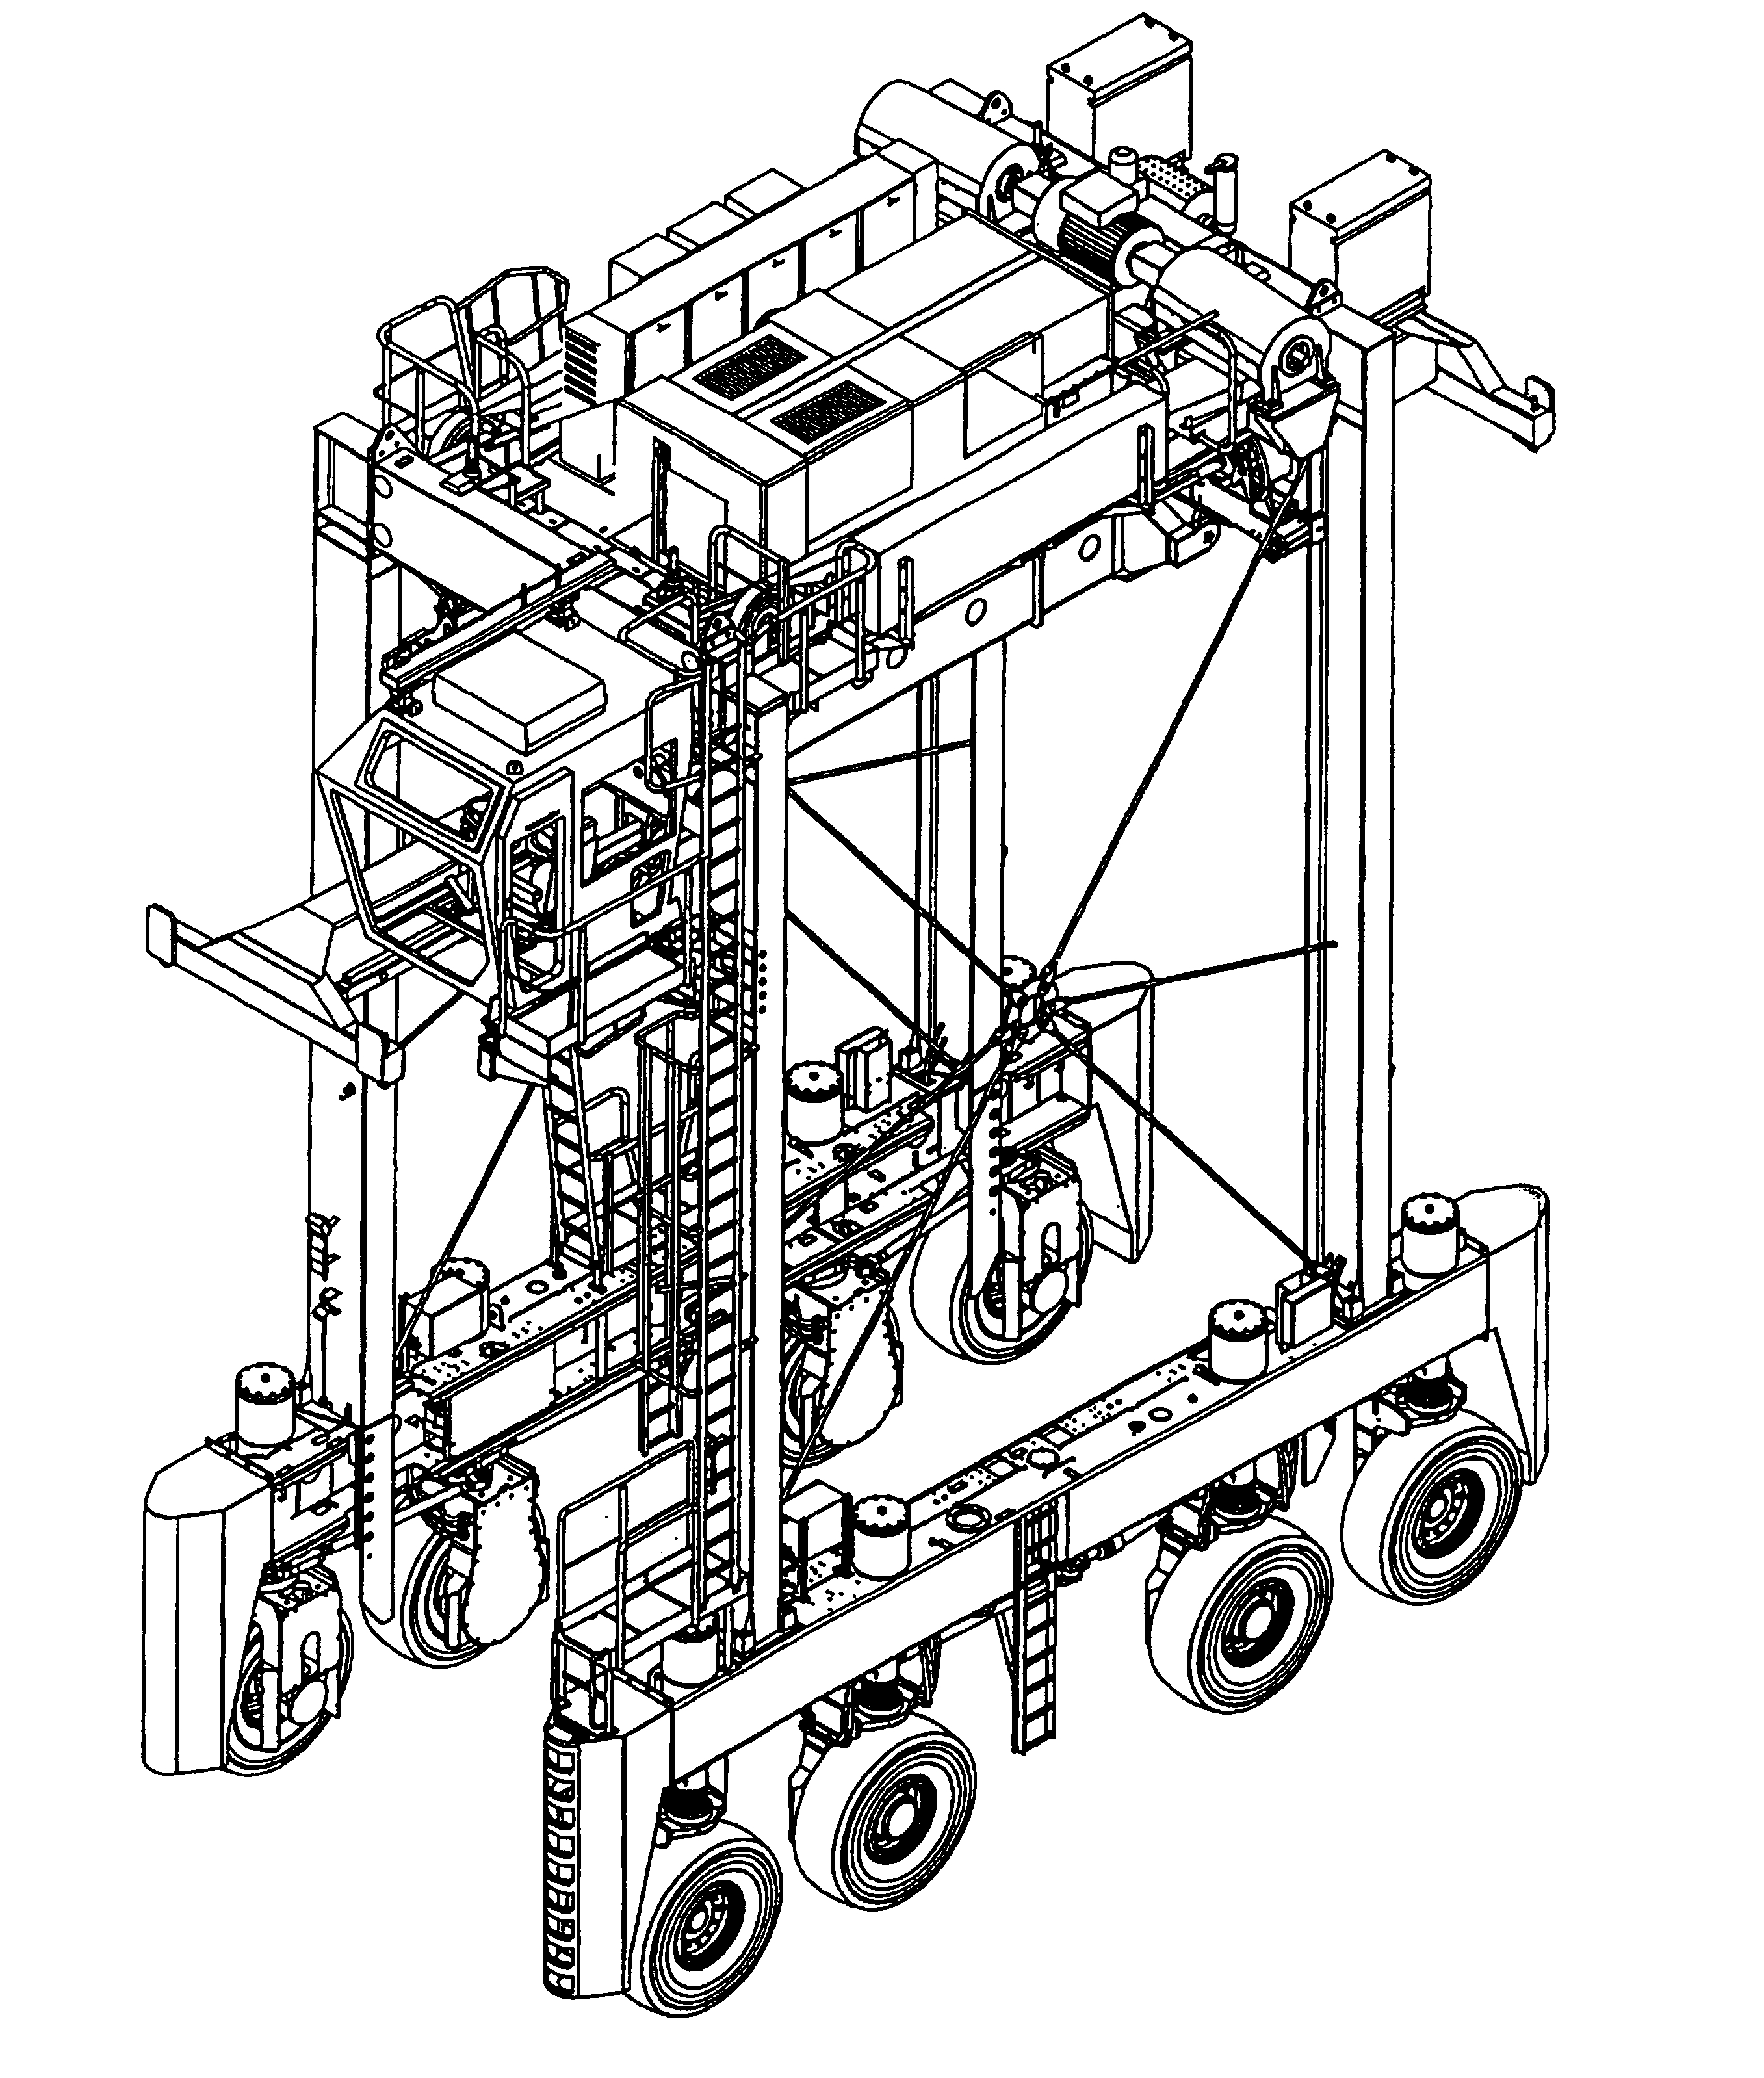
\includegraphics[height=.25\textheight]{fig/schema_sc.jpg}
    \end{column}
    \begin{column}[c]{4.0cm}	
      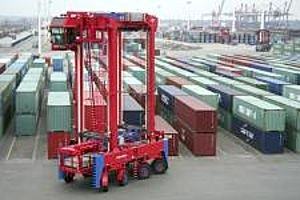
\includegraphics[height=.25\textheight]{fig/chariot_cavalier.jpg}
    \end{column}
    \begin{column}[r]{3.0cm}	
      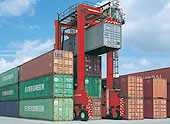
\includegraphics[height=.25\textheight]{fig/tn-straddle-carriers.jpg}
   \end{column}
\end{columns}
  \end{center}
\begin{itemize}
   \pause \item sur les routes : les chariots peuvent se croiser et se doubler 
   \pause \item sur les travées : les chariots ne peuvent ni se croiser ni se doubler
 \end{itemize}
\begin{center}
\pause $\Rightarrow$ Les travées sont modélisés par des arcs FIFO
 \end{center}
 \end{frame}

  \subsection{Temporalité}
\begin{frame}{Temporalité}  
  \begin{itemize}
   \item Le temps a été discrétisé
   \item La durée d'un pas de temps est définie avant le lancement de la simulation
  \end{itemize}  
\end{frame}

\begin{frame}{Exemple : terminal après 2 itérations (1 itération = 1s)}
 \begin{columns}
    \begin{column}[l]{6.5cm}	
\begin{center}  
    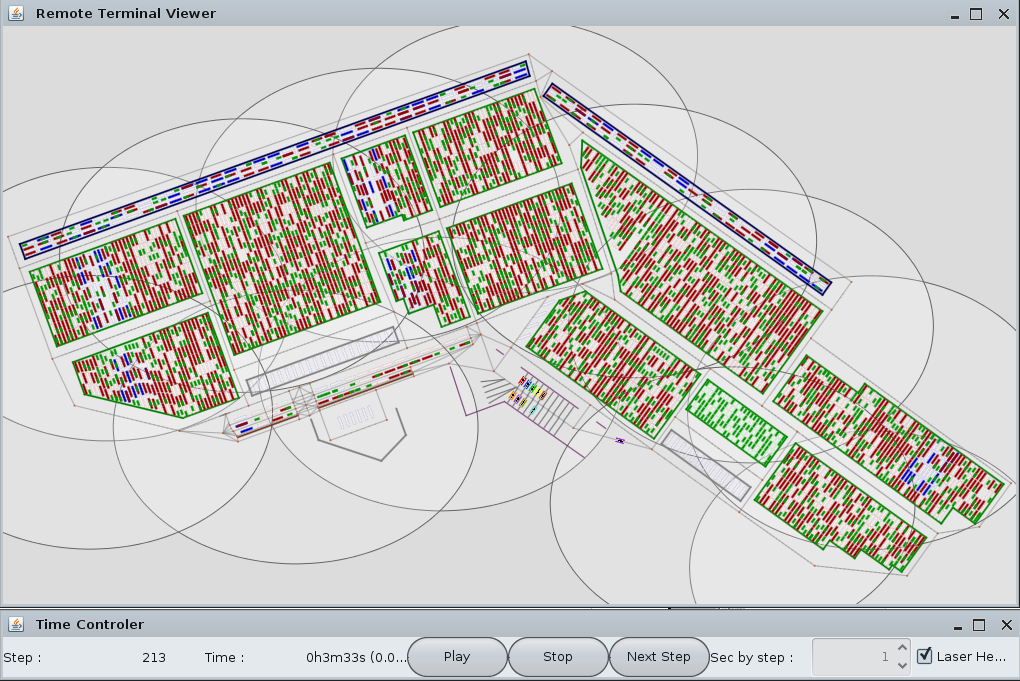
\includegraphics[width=.85\textheight]{fig/capture3m33s.png}
\end{center}
    \end{column}
   
    \begin{column}[r]{6.5cm}	
\begin{center}      
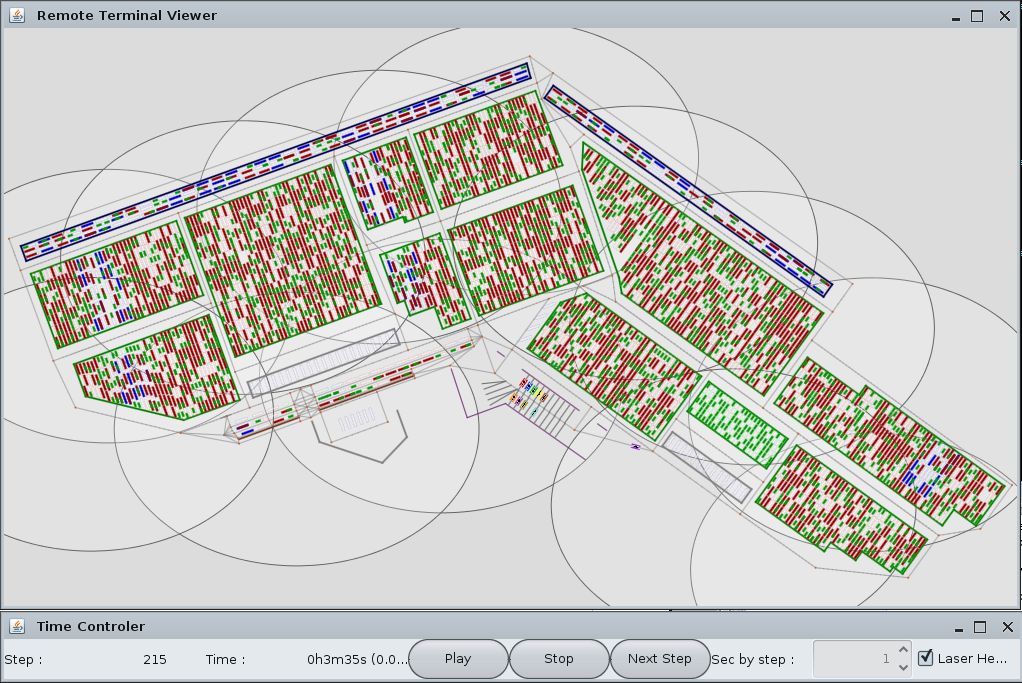
\includegraphics[width=.85\textheight]{fig/capture3m35s.png}
\end{center}
   \end{column}
\end{columns}
\end{frame}

  \subsection{Évenements}
  \begin{frame}{Les événements}
   \begin{itemize}
    \item Arrivée de mission
    \pause
    \item Arrivée/départ de véhicule
    \pause
    \item Panne (ou réparation) de chariot cavalier
    \pause
    \item Non respect d'affectation de mission d'un chariot cavalier
    \pause
    \item Non respect d'itinéraire d'un chariot cavalier
    \pause
    \item Perte de conteneur
    \pause
    \item Panne de borne laser (complete ou perte de portée)
   \end{itemize}
  \end{frame}

\section{Collecte et structure des données}
 
\begin{frame}{Collecte des données}
    Plan fourni par nos partenaires
    \begin{center}
      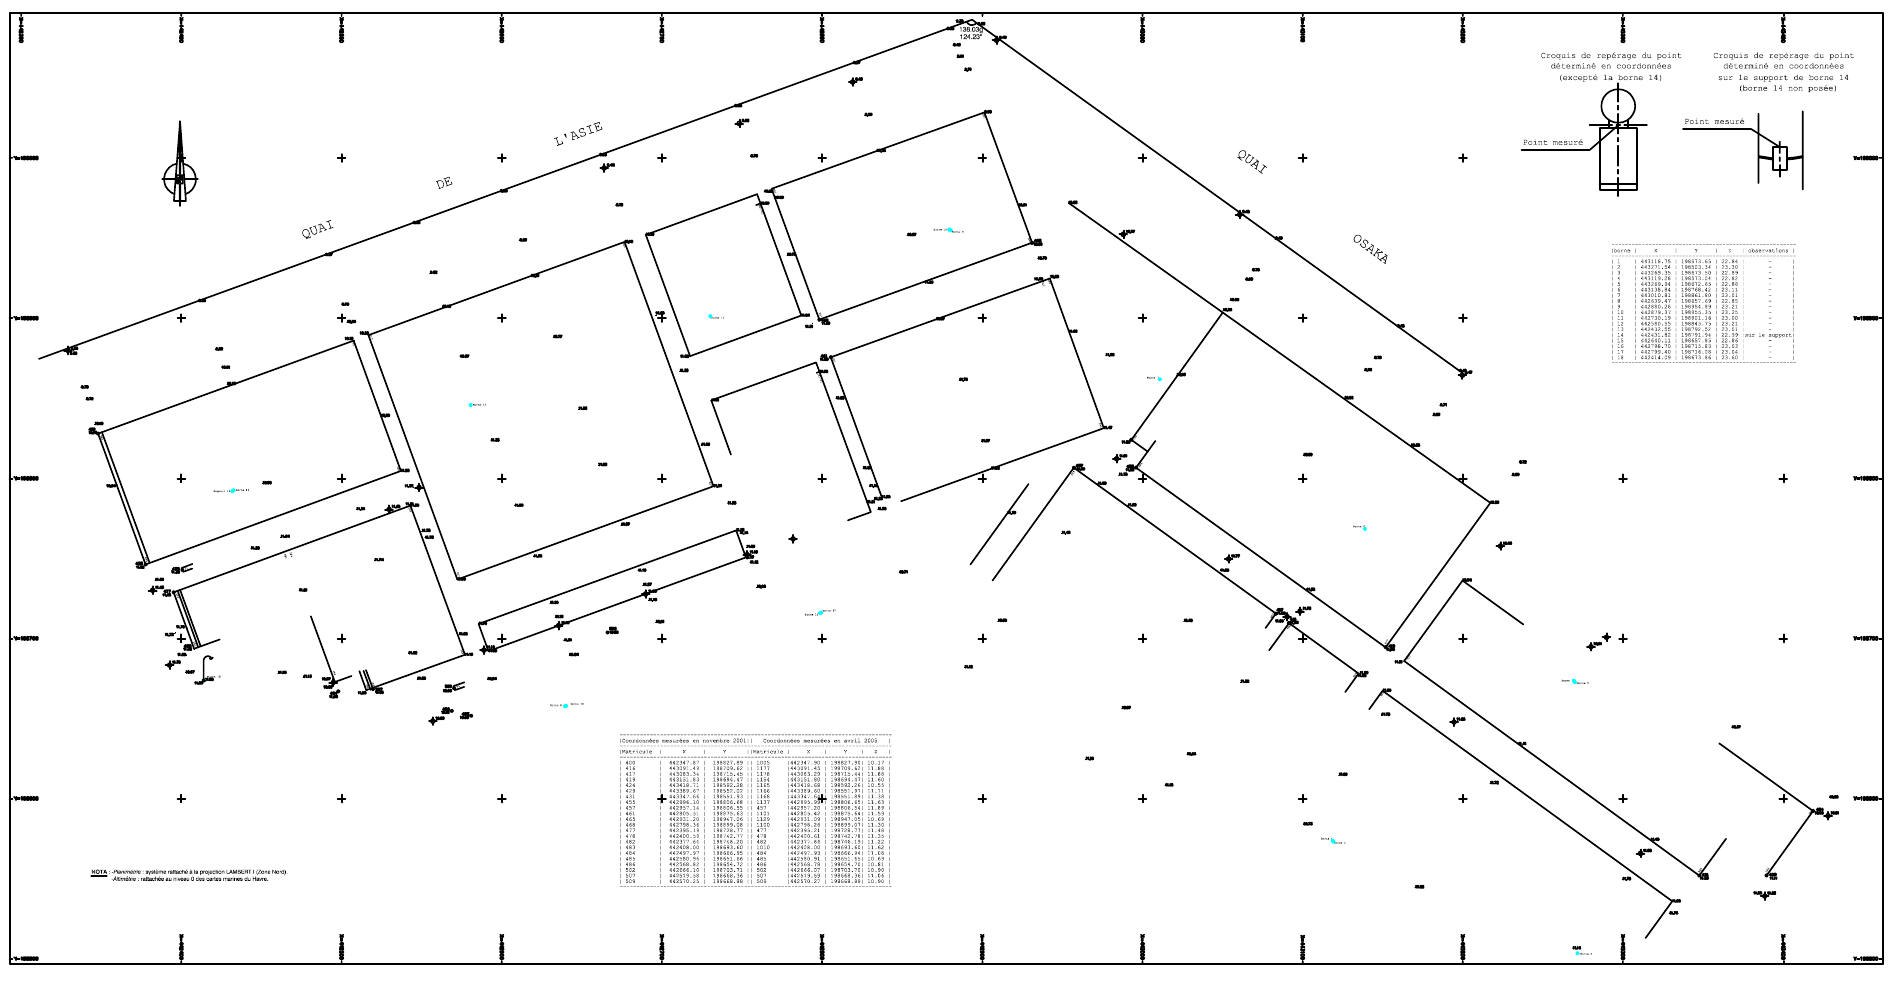
\includegraphics[height=.70\textheight]{fig/planNormandieZ.png}
    \end{center}
\end{frame}
\begin{frame}{Collecte des données (2)}
    Collecte de données à partir d'images satellites (www.wikimapia.org)
    \begin{center}
      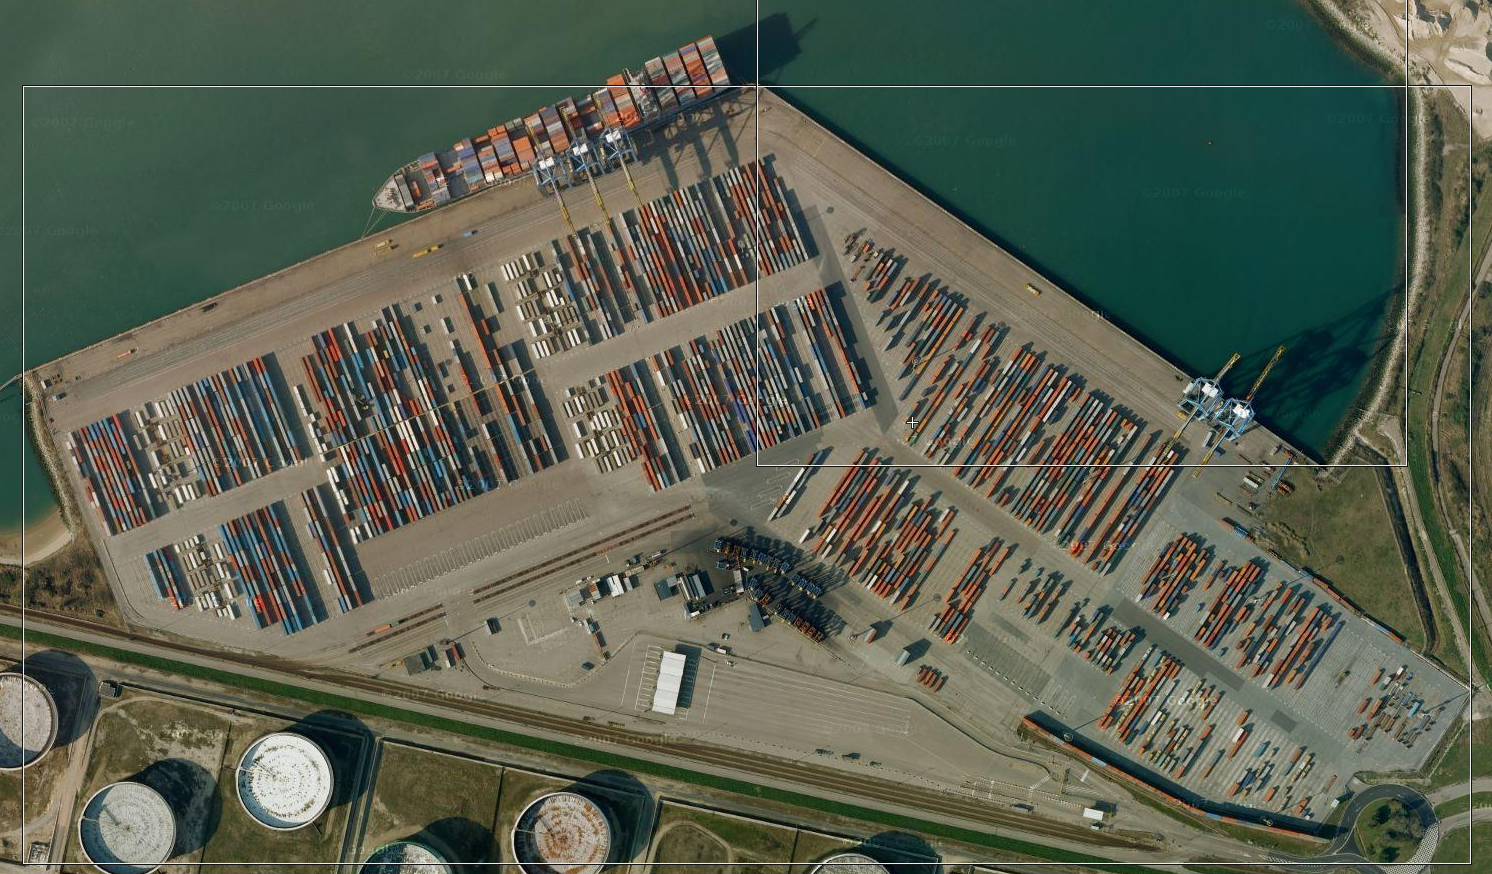
\includegraphics[height=.70\textheight]{fig/NormandieZ.png}
    \end{center}
\end{frame}
\begin{frame}{Structuration des données}
  
  \begin{block}{Structure XML}
    \begin{itemize}
      \item Clarté des données
      \item Personnalisation
      \item Navigation facilité
    \end{itemize}
   \end{block}
   
  \begin{center}   
    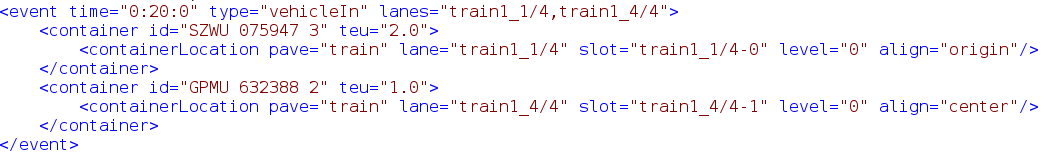
\includegraphics[width=.90\textwidth]{fig/structureXML.png}
   \end{center}
\end{frame}

\begin{frame}{Résultat de la collecte et de la structuration des données}
    Création d'un plan détaillé
    \begin{center}
      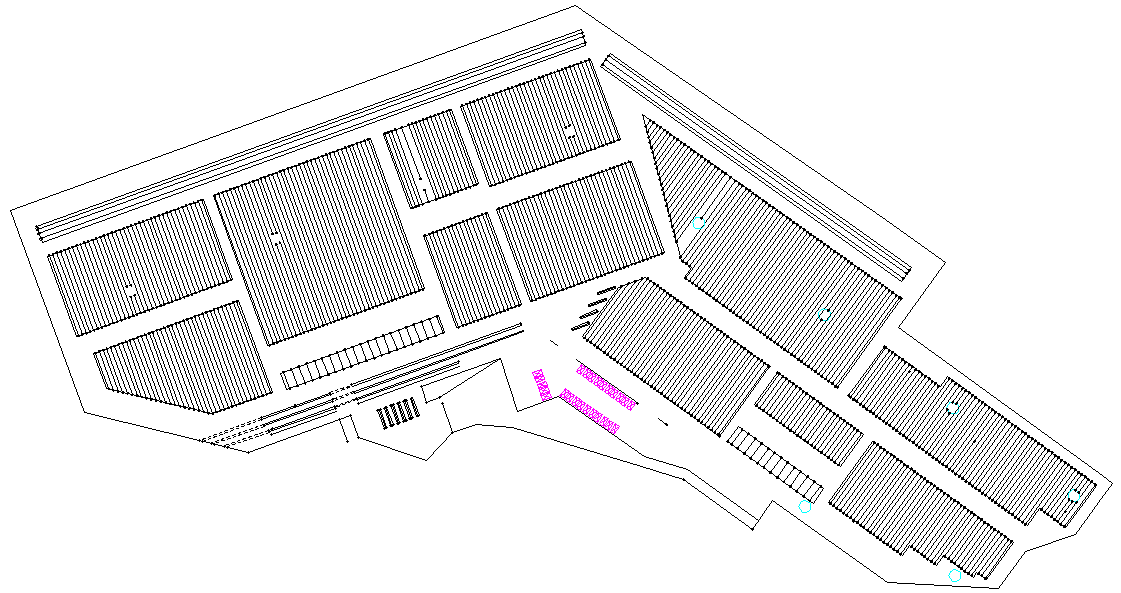
\includegraphics[height=.70\textheight]{fig/planTerminalDetailleBlanc.png}
    \end{center}
\end{frame} 
\section{Les problèmes simulés}
\subsection{Architecture du terminal}
\begin{frame}{Configuration d'un terminal}
  \begin{block}{Objectif :}
    Tester la structure d'un terminal
  \end{block}
  \pause
  Mesurer l'impact de l'architecture du terminal sur : 
  \begin{itemize}
  \pause
   \item Les coûts d'exploitation
  \pause
   \item La qualité de service
  \end{itemize}
 \end{frame}
\subsection{Positionnement des conteneurs dangereux}
\begin{frame}{Positionnement des conteneurs dangereux}
  \begin{block}{Objectif :}
    Déterminer l'emplacement de stockage d'un conteneur dangereux
  \end{block}
  \pause
  Le problème consiste à choisir un emplacement permettant de réduire les distances de manutention du conteneur tout en assurant le respect des normes de sécurités
 \end{frame}
    \subsection{Ordonnancement de missions}
\begin{frame}{Ordonnancement dynamique}
 \begin{itemize}   
   \item Pour un chariot cavalier, une mission consiste à déplacer un conteneur.
   \pause
    \item 3 types de mission : 
    \begin{itemize}
      \item Chargement de navire, train, ou camion
      \item Déchargement de navire, train, ou camion
      \item Optimisation de la zone de stockage
    \end{itemize}
    \pause
    \item 2 phases : collecte et livraison
    \pause
    \item 2 fenêtres de temps 
    \pause
    \item $m$ chariots cavaliers
    \item $n$ missions
\end{itemize}
\pause
\begin{block}{ Problème modélisé : }
   	\begin{minipage}[]{\columnwidth}
		Version dynamique d'un problème d'ordonnancement et d'affectation de missions
	\end{minipage}
  \end{block}
  \end{frame}
\subsection{Routage des véhicules}
\begin{frame}{Problème de routage}
    \begin{block}{Problème classique : }
      Minimiser la distance parcourue par les chariots cavaliers pour réduire les coûts d'exploitation
    \end{block}
\pause
    \begin{block}{Problème de routage sur un terminal :}
       \begin{itemize} 
	  \item Routes : arcs non FIFO
	  \item Travées : arcs FIFO a capacité unitaire
	  \item La vitesse d'un chariot cavalier dépend de sa position
	
	\end{itemize}
	\pause
	\begin{center}
	    $\Rightarrow$ Minimiser les temps de parcours pour réduire les coûts et maintenir une qualité de service suffisante	  
	  \end{center}
    \end{block}
  \end{frame}

\section{Démonstration}
  \begin{frame}{Démonstration}
    \begin{block}{Données de la simulation : }
     \begin{itemize}
      \item Terminal de Normandie (Port Autonome du Havre)
      \item 1h simulée
      \item 52 missions
      \item 10 chariots cavaliers
      \item Ordonnancement aléatoire
     \end{itemize}
    \end{block}
  \end{frame}

  \begin{frame}{Conclusion}
    \begin{itemize}
     \item Le simulateur est presque achevé
    \pause
     \item Collaboration avec EADS/Astrium pour intégrer un module de visualisation 3D
    \pause
     \item Recherche de partenaires pour : 
	\begin{itemize}
	 \item collecter des données (structures de terminaux, jeux de tests)
	 \item tester des algorithmes (ordonnancement de missions, routage des chariots)
	\end{itemize}
    \end{itemize}
  \pause
  \begin{center}
  contact : gaetan.lesauvage@litislab.eu
  \end{center}
  \end{frame}
\end{document}
